\documentclass[12pt,a4paper,titlepage]{article}
%\usepackage[hmargin=3cm,vmargin=3.5cm]{geometry}
\usepackage[latin1]{inputenc}
\usepackage{amsmath}
\usepackage{amsfonts}
\usepackage{amssymb}
\usepackage{graphicx}
\usepackage{listings}
\usepackage{datetime}
\usepackage{url}
\usepackage{hyperref}
\usepackage{gensymb}

\author{}
\title{Puma for FreeEMS\newline Assembly, configuration, modification and installation manual}

\begin{document}
\maketitle
\pagebreak

\tableofcontents
\thispagestyle{empty}
\pagebreak

\section{Overview}

This document is to show how to choose components to order, properly build and connect your Spin 1 board to a vehicle.

Puma uses FreeEMS vanilla firmware, PC tuning software and Puma hardware to control fuel and ignition of large variety of engine configurations. See \url{http://puma.freeems.org} for a more detailed overview of what PUMA can do and is used for. 

We recommend you purchase the hardware such that many of the below steps aren't required. This version of the manual includes instructions for the Spin 1 board, which was generally provided as just a bare board. You will need to purchase parts based on a BOM then install those parts. You will also need to program the board via BDM programming port to get the initial bootloader installed. After the initial build, you will be able to program the board with an USB cable and a standard PC.

Note these sections are written as modules, such that sections are useful on their own, but also arranged in a sequence that is handy for a first time installer. 

\section{Getting the hardware}

The design and software is OpenSource and while you can technically build it by yourself, we recommend you purchase PUMA assembled. This is how you get the hardware, blah blah blah.

Spin 1 offered just the bare board, so there are notes about how to do some low level assembly, but future spins will likely remove these assembly notes. 

\section{So you have a bare board, now what?}

Ok, you have the bare PCB, and it's going to need components installed on it to function as a EMS. This is what you need to do, in no particular order:
\begin{itemize}
\item Get the BOM from site, its in csv format, so you can select what modules you want populated.
A few things to note:
EGT circuit won't work, it has a 500$^{\circ}$C limit.
The usb connector is plain wrong. In the BOM you can choose to buy a cable to use this wrong (female-A) connector, or buy another usb connector and hack things to install it.
You don't want the shutdown circuit, so its FETs aren't in the BOM. Don't worry about that.

Once you are decided about the BOM, go to to digikey and place the order.

\item Modify the board as shown in ``Spin 1 specific notes"

We recommend doing these steps sequentially.

\begin{enumerate}
\item Install MCU and critical components.
\item Test the MCU works by uploading the firmware
\item Install rpm input circuit choose hall input, or VR
\item Install misc outputs like Fuel, ect
\item Install injectors circuits
\item Install ignitions circuits
\end{enumerate}

\end{itemize}

\subsection{You now have a PUMA board with components, now what?}

You will likely want to verify the board is good with a Jim Stim  then it will need the initial firmware installed. If PUMA was purchased assembled, these steps should not be required, and you can proceed to the next step.

\subsection{Testing your board with Jim Stim.}

Blah blah blah, fill in this stuff.

\subsection{Uploading the initial firmware.}

BDM loader notes and more blah blah blah. 
 

\section{Connecting the board to a vehicle}

Figure~\ref{fig:wiring} shows how the PUMA board should be connected to the engine.

\begin{figure}[htb]
\begin{center}
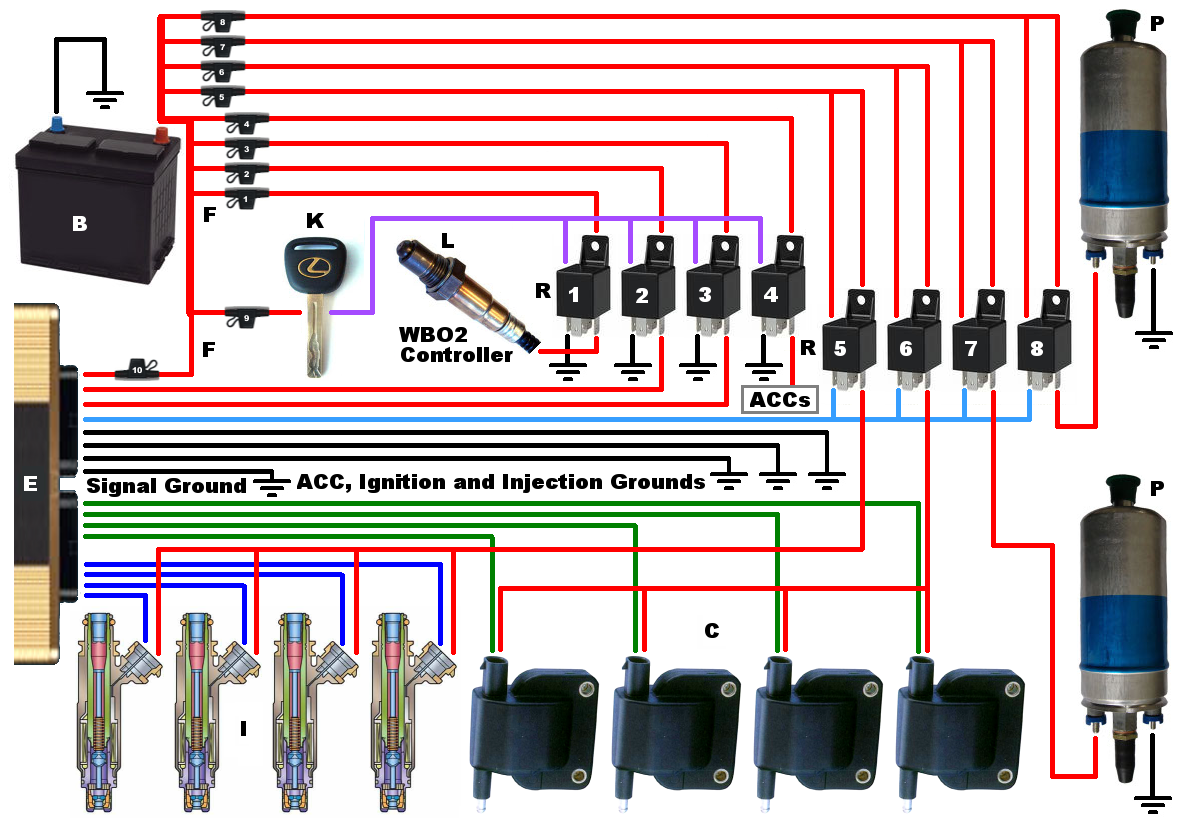
\includegraphics[width=1\textwidth]{images/freeems-power-wiring5.png}
\caption{Wiring diagram}
\label{fig:wiring}
\end{center}
\end{figure}

\section{Uploading firmware via USB and boot loader}

So you have a PUMA that may or may not be connected to your system.

This is how to upload a new firmware file to that board.

\begin{itemize}
\item Download and install 

\item Open

\item Configure USB port

\item Specify to upload firmware file.
\end{itemize}


\section{Trying out the board with a Tuning Software}

If you have engine setup blah, this is the basic way to tune your engine.
If you have engine setup blah2, this is the way you tune your engine.

\section{Spin1 specific notes}

\begin{enumerate}
\item This spin has several modifications. Start these modifications by cut the wrong traces, and adding jumpers as shown below.

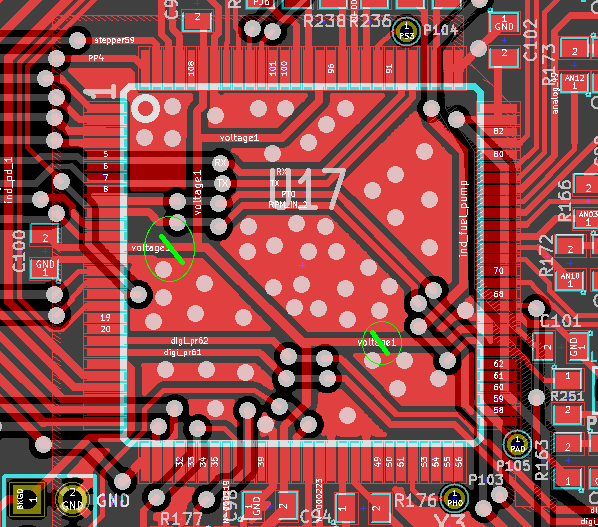
\includegraphics[width = 6cm]{images/MCU_VDD_traces.png}

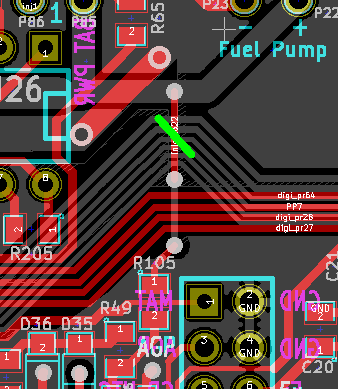
\includegraphics[width = 6cm]{images/BRV_hack.png}

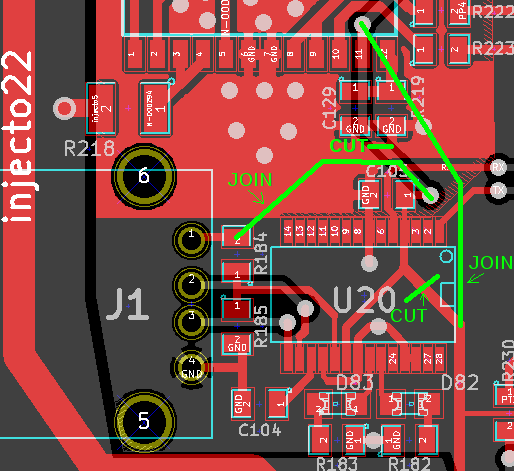
\includegraphics[width = 6cm]{images/USB_power_hack.png}

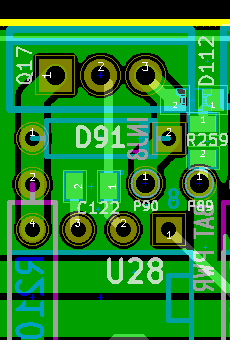
\includegraphics[width = 6cm]{images/P&H_hack.png}

\item You have the PCB + components, so get KICAD and the files, or the pdf files from puma.freeems.org. PDFs aren't search-able so you may want to choose to install KICAD until we workout that.

\item Start the assembly!

Just solder the components. If you ordered a board, you should know how to do it. An oven is a fast way to get it done.

Don't put too much paste for the small regulator, or it will get misaligned.

Components that shouldn't be populated:

\begin{itemize}
\item F1, F3 (Fuses)
\item R226, R227, Q18, Q19, bridge pin 1 and 3 of Q19 (this is the shutdown circuit)
\item R133 (bad pullup)
\item R228 OR R229, using one of them defines whether the XOR negates or not its outputs.
\item If you use VR inputs, R212, R213, R215, and R216 should be bigger, like $\frac{1}{4}$ or $\frac{1}{2}$W. 10k\ohm to 20k\ohm will be fine.
\item U18, R186, R187, C107, D74, D75, C106 (thermocouple driver)
\end{itemize}

\item Program the MCU using a BDM pod.

Install Codewarrior, open the programmer, go to File $\rightarrow$ Load application, and select the .s12 (FreeEMS serial monitor).

It should get connected, program it, verify, and never complain.

\item Load FreeEMS firmware, using seank's loader.

\item Install  MTX and connect to the board to the PC to check that freeems is running.

\end{enumerate}



\end{document}


